\section{Calibration des observations photométriques}
% Description des étapes du traitement et discussion de leurs effets.
Maintenant que nous avons rapidement introduit les paramètres de notre capteur CCD ainsi que de nos acquisitions, nous allons pouvoir présenter les différentes étapes nécessaire à la calibration de nos mesures photométriques. En effet, nous avons précédemment établi la formule \textbf{REFERENCE A AJOUTER} nous permettant de relier le flux de chaque étoile à sa magnitude, or dès lors que nous procédons à des mesures expérimentales, le flux que nous récupérons pour chaque étoiles dépend de nombreux facteurs que nous allons tenter d'explorer dans la présente section, en commençant par les critères qui vont définir la détection des sources présentes sur notre image. Notons ici rapidemment que comme nous l'avons évoqué précedemment, nous avons travaillé durant cette étude sur deux types de filtres différents. Ceux-ci n'ayant pas d'impact sur le choix des paramètres de calibration en eux-mêmes, nous avons utilisé durant cette partie les données du filtre $r$, et nous transposerons nos choix sur les données filtre $g$ lorsque nous étudierons les mesures finalement réalisées. 

\subsection{Critères de détections}
Les critères de détection qui sont utilisés pour détecter des sources sur une image CCD sont assez directement liées à l'outil utilisé pour effectuer cette détection, bien que gloabalement, les notions seront toujours les mêmes. Dans notre cas, nous effectuons cette détection à l'aide de la librairie Python \textit{Photutils}, et celle-ci prend comme arguments les paramètres suivants:

\begin{itemize}
  \item La largeur à mi-hauteur
  \item{Le pic maximum} 
  \item{Le seuil de détection} 
\end{itemize}

\noindent Nous allons donc rapidement décrire chacun de ces paramètres et justifier comment nous les avons déterminés. \\

En premier donc, la largeur à mi-hauteur (ou FWHM, de l'anglais Full Width at Half Maximum) est un paramètre permettant de caractériser "l'étalement" de nos sources sur notre capteur CCD, et est donc directement lié à la fonction d'étalement du point de notre acquisition (ou PSF de l'anglais Point Spread Function). En astrophotométrie, nous étudions des sources à des distances telles que celle-ci sont théoriquement ponctuelles pour les capteurs que nous utilisons, c'est-à-dire que leur taille réelle est inférieure à la résolution instrumentale, or dans la pratique le trajet optique dans l'atmosphère ainsi que dans les lentilles du téléscope et du capteur va avoir pour effet de diffuser les photons reçus, "étalant" ces derniers sur plusieurs pixels du capteur. Cet étalement est donc caractérisé par la PSF (la convolution de la PSF et de la source "réelle" résulte en l'image finalement produite par le capteur) et varie pour chaque acquisition, tandis qu'elle est supposée être constante à travers une même image. Ce dernier point nous permet donc d'établir un critère de définition de la largeur à mi-hauteur: celle-ci étant la même sur toute notre image, nous allons prendre une source possédant un excellent rapport signal/bruit (nous reviendrons plus tard en détail sur cette notion, comprendre ici qu'il s'agit d'un des meilleurs rapports signal/bruit que nous avons parmis nos sources) et l'utiliser pour déterminer avec le plus de précision possible la forme que les sources auront sur notre notre image. Nous avons pour cela observé en 3D les électrons mesurés par le capteur en fonction de leur position sur celui-ci:

\begin{figure}[h]
        \centering
        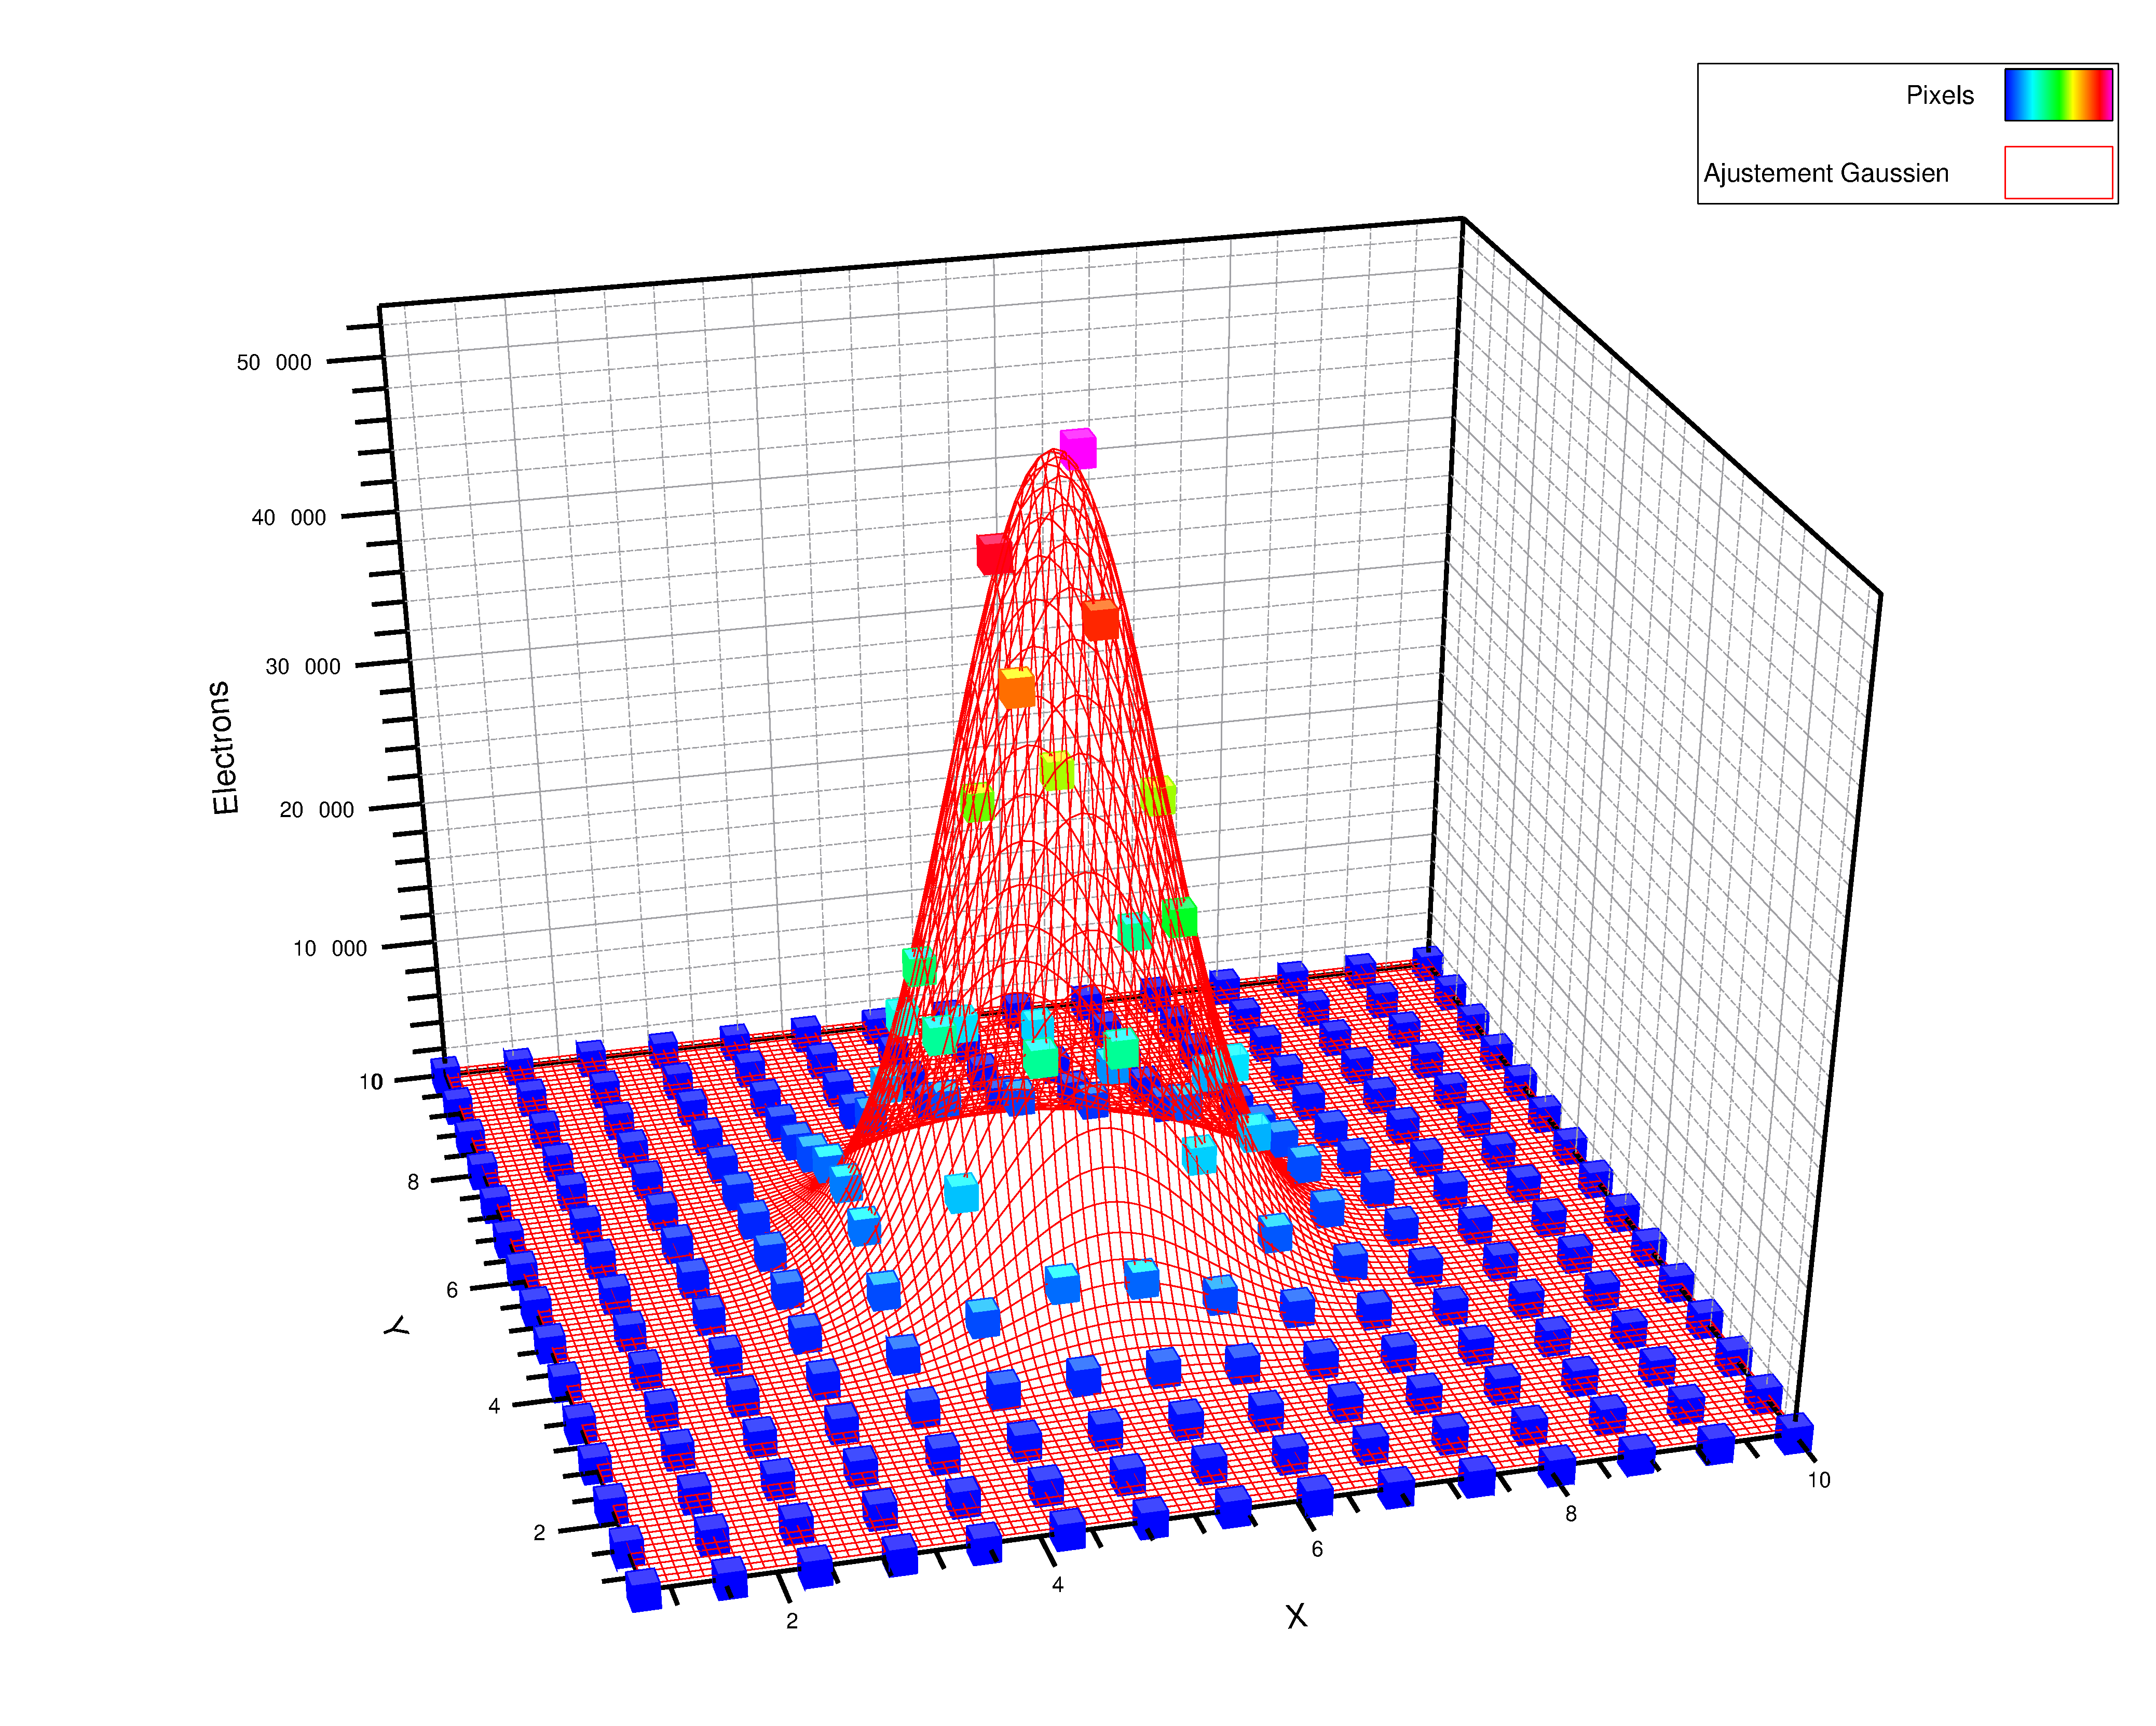
\includegraphics[width=0.7\linewidth]{fig/FWHM.pdf}
        \caption{Visualisation des photons mesurés pour une étoile avec un important rapport signal/bruit\label{fwhm}}
\end{figure}

\noindent Ici apparaît clairement que la source n'est effectivement pas parfaitement ponctuelle, et que le flux mesuré par le capteur est réparti sur plusieurs pixels. Nous avons également superposé un ajustement selon une Gaussienne en 3D, modèle le plus proche de nos valeurs, et permettant donc de justifier l'utilisation du terme de FWHM, que nous avons donc déterminé à partir de cette modélisation. Il est important de relever qu'à partir du moment où l'on considère une gausienne en 3D, la notion de FWHM dépend de la direction ($x$ ou $y$), le rapport entre ces deux FWHM définit même la rondeur $r$ de l'étoile (plus $r$ est proche de 1, plus l'étoile est dite ronde). Dans notre cas cependant, la rondeur est de $r=1.009$, nous allons donc pendant notre étude considérer nos sources comme parfaitement rondes et prendront la moyenne des deux FWHM comme paramètre de détection. Nous avons donc à partir des paramètres de modélisation déterminés par $Qtiplot$ obtenus une largeur à mi-hauteur de:

\[\boxed{\text{FWHM}=1.95 \; \text{pixels}}\]

\noindent Nous considérerons cette grandeur comme sans incertitude, celle-ci étant trop délicate à implémenter dans notre fonction de détection de sources, et de toute manière très faible grâce au choix d'une étoile avec un important rapport signal/bruit (on s'attend à ce que son profil soit le plus proche possible de la PSF de notre acquisition). \\

Le prochain paramètre que nous allons aborder est celui du pic maximum. Celui-ci est relié au profil de nos sources que nous venons de décrire, le pixel qui va détecter le point central de la PSF va donc mesurer la plus grande valeur en électrons (dans le cas idéal ou ce point est centré sur un pixel, il peut également tomber entre plusieurs pixels et dans ce cas on observera plusieurs pixels qui auront des valeurs proches du pic). Cette valeur de pic nous permet donc de définir un critère de sélection des sources, car nous cherchons à éviter de travailler avec des sources qui auraient saturé le capteur, car nous perdrions de l'information et cela mènerait à des mesures fausses. Nous voyons sur la Table \ref{CCD} que la capacité maximale de notre capteur est de $10 ^{5} e-$, soit environ $65000$ ADU. Nous avons choisi de définir ce critère de saturation à $50 000$ ADU, car nous avons très peu de sources au-delà de cette valeur, nous en excluons donc une faible quantité tout en étant ainsi sûr d'être suffisamment loin du niveau de saturation du capteur. Le gain permettant de convertir les électrons mesurés en ADU, nous posons finalement le pic maximum comme:

\[\boxed{\text{Pic Maximum} = \text{Gain}*50 000 \; \text{électrons}}\]

Finalement, le dernier critère de détection que nous devons considérer est celui du "seuil" ("treshold" en anglais), soit la valeur à partir de laquelle un pixel sera considéré comme une source. Celle-ci est généralement exprimée comme un multiple de la valeur du fond de ciel, sur lequel nous allons revenir plus en détail, mais qui correspond à la valeur mesurée par le CCD en dehors des sources elles-même. Une valeur trop proche de celle du fond de ciel signifie que l'on considérera par erreur des pixels chauds ou de simples variations du fond comme des sources, tandis qu'une valeur trop haute implique que nous considérerons simplement moins d'étoiles, ce paramètre peut donc dans notre cas être utilisé pour sélectionner plus ou moins d'étoiles, en considérant que nous plus ce paramètre baisse, plus les nouvelles étoiles détéctées auront un flux faible, ainsi on s'attend à globalement ajouter des étoiles avec un moins bon rapport signal bruit en baissant le seuil. En jouant sur ce paramètre, nous avons choisi un paramètre arbitrairement, nous permettant de détecter un nombre de source suffisant pour effectuer une bonne calibration sans avoir de risque de détecter de "faux positifs":

\[\boxed{\text{Seuil}=\text{Fond de ciel}*100 \; \text{électrons}}\]

\subsection{Méthodes d'annulation du fond de ciel\label{Label}}%
Maintenant que nous avons établis les paramètres avec lesquels nous détectons nos sources, discutons de la méthode que nous allons utiliser pour déterminer la valeur du fond de ciel de notre image. Nous avons à notre disposition 
  
\subsection{Rayon d'ouverture optimal}
\subsubsection{Notion de rapport signal/bruit\label{Label}}%
\subsubsection{Critère du RSB le plus faible\label{Label}}%
\subsubsection{Critère RSB sur chaque étoile\label{Label}}%
\subsubsection{Méthode d'optimisation Flux-RSB\label{Label}}%
\subsubsection{Impact de chaque méthodes sur la calibration\label{Label}}%
  
  
\subsection{Calibration en fonction des paramètres idéaux déterminés\label{Label}}%
  
  
  
\section{Mesures photométriques et incertitudes}

\subsection{Mesures de magnitudes (filtre r)\label{Label}}%

\subsection{Mesure de magnitudes (filtre g)\label{Label}}%
  
  
% Pour les projets de spectroscopie : mesures de longueur d'onde, largeur équivalente, vitesse radiale, identification de raies spectrales
% Pour les projets de photométrie : mesure photométriques sur les étoiles cibles/références
